\documentclass[twoside]{book}

% Packages required by doxygen
\usepackage{fixltx2e}
\usepackage{calc}
\usepackage{doxygen}
\usepackage[export]{adjustbox} % also loads graphicx
\usepackage{graphicx}
\usepackage[utf8]{inputenc}
\usepackage{makeidx}
\usepackage{multicol}
\usepackage{multirow}
\PassOptionsToPackage{warn}{textcomp}
\usepackage{textcomp}
\usepackage[nointegrals]{wasysym}
\usepackage[table]{xcolor}

% Font selection
\usepackage[T1]{fontenc}
\usepackage[scaled=.90]{helvet}
\usepackage{courier}
\usepackage{amssymb}
\usepackage{sectsty}
\renewcommand{\familydefault}{\sfdefault}
\allsectionsfont{%
  \fontseries{bc}\selectfont%
  \color{darkgray}%
}
\renewcommand{\DoxyLabelFont}{%
  \fontseries{bc}\selectfont%
  \color{darkgray}%
}
\newcommand{\+}{\discretionary{\mbox{\scriptsize$\hookleftarrow$}}{}{}}

% Page & text layout
\usepackage{geometry}
\geometry{%
  a4paper,%
  top=2.5cm,%
  bottom=2.5cm,%
  left=2.5cm,%
  right=2.5cm%
}
\tolerance=750
\hfuzz=15pt
\hbadness=750
\setlength{\emergencystretch}{15pt}
\setlength{\parindent}{0cm}
\setlength{\parskip}{3ex plus 2ex minus 2ex}
\makeatletter
\renewcommand{\paragraph}{%
  \@startsection{paragraph}{4}{0ex}{-1.0ex}{1.0ex}{%
    \normalfont\normalsize\bfseries\SS@parafont%
  }%
}
\renewcommand{\subparagraph}{%
  \@startsection{subparagraph}{5}{0ex}{-1.0ex}{1.0ex}{%
    \normalfont\normalsize\bfseries\SS@subparafont%
  }%
}
\makeatother

% Headers & footers
\usepackage{fancyhdr}
\pagestyle{fancyplain}
\fancyhead[LE]{\fancyplain{}{\bfseries\thepage}}
\fancyhead[CE]{\fancyplain{}{}}
\fancyhead[RE]{\fancyplain{}{\bfseries\leftmark}}
\fancyhead[LO]{\fancyplain{}{\bfseries\rightmark}}
\fancyhead[CO]{\fancyplain{}{}}
\fancyhead[RO]{\fancyplain{}{\bfseries\thepage}}
\fancyfoot[LE]{\fancyplain{}{}}
\fancyfoot[CE]{\fancyplain{}{}}
\fancyfoot[RE]{\fancyplain{}{\bfseries\scriptsize Generated by Doxygen }}
\fancyfoot[LO]{\fancyplain{}{\bfseries\scriptsize Generated by Doxygen }}
\fancyfoot[CO]{\fancyplain{}{}}
\fancyfoot[RO]{\fancyplain{}{}}
\renewcommand{\footrulewidth}{0.4pt}
\renewcommand{\chaptermark}[1]{%
  \markboth{#1}{}%
}
\renewcommand{\sectionmark}[1]{%
  \markright{\thesection\ #1}%
}

% Indices & bibliography
\usepackage{natbib}
\usepackage[titles]{tocloft}
\setcounter{tocdepth}{3}
\setcounter{secnumdepth}{5}
\makeindex

% Hyperlinks (required, but should be loaded last)
\usepackage{ifpdf}
\ifpdf
  \usepackage[pdftex,pagebackref=true]{hyperref}
\else
  \usepackage[ps2pdf,pagebackref=true]{hyperref}
\fi
\hypersetup{%
  colorlinks=true,%
  linkcolor=blue,%
  citecolor=blue,%
  unicode%
}

% Custom commands
\newcommand{\clearemptydoublepage}{%
  \newpage{\pagestyle{empty}\cleardoublepage}%
}

\usepackage{caption}
\captionsetup{labelsep=space,justification=centering,font={bf},singlelinecheck=off,skip=4pt,position=top}

%===== C O N T E N T S =====

\begin{document}

% Titlepage & ToC
\hypersetup{pageanchor=false,
             bookmarksnumbered=true,
             pdfencoding=unicode
            }
\pagenumbering{alph}
\begin{titlepage}
\vspace*{7cm}
\begin{center}%
{\Large Y\+O\+U\+S\+S\+EF }\\
\vspace*{1cm}
{\large Generated by Doxygen 1.8.13}\\
\end{center}
\end{titlepage}
\clearemptydoublepage
\pagenumbering{roman}
\tableofcontents
\clearemptydoublepage
\pagenumbering{arabic}
\hypersetup{pageanchor=true}

%--- Begin generated contents ---
\chapter{Data Structure Index}
\section{Data Structures}
Here are the data structures with brief descriptions\+:\begin{DoxyCompactList}
\item\contentsline{section}{\hyperlink{structent}{ent} \\*Struct for entite }{\pageref{structent}}{}
\end{DoxyCompactList}

\chapter{File Index}
\section{File List}
Here is a list of all documented files with brief descriptions\+:\begin{DoxyCompactList}
\item\contentsline{section}{\hyperlink{afficher__entite_8c}{afficher\+\_\+entite.\+c} }{\pageref{afficher__entite_8c}}{}
\item\contentsline{section}{\hyperlink{anim__entite__droite_8c}{anim\+\_\+entite\+\_\+droite.\+c} }{\pageref{anim__entite__droite_8c}}{}
\item\contentsline{section}{\hyperlink{animate__enemy_8c}{animate\+\_\+enemy.\+c} }{\pageref{animate__enemy_8c}}{}
\item\contentsline{section}{\hyperlink{dep__va__x_8c}{dep\+\_\+va\+\_\+x.\+c} }{\pageref{dep__va__x_8c}}{}
\item\contentsline{section}{{\bfseries entite.\+h} }{\pageref{entite_8h}}{}
\item\contentsline{section}{\hyperlink{free__enemy_8c}{free\+\_\+enemy.\+c} }{\pageref{free__enemy_8c}}{}
\item\contentsline{section}{\hyperlink{init__entite_8c}{init\+\_\+entite.\+c} }{\pageref{init__entite_8c}}{}
\item\contentsline{section}{\hyperlink{main_8c}{main.\+c} }{\pageref{main_8c}}{}
\item\contentsline{section}{\hyperlink{move__enemy_8c}{move\+\_\+enemy.\+c} }{\pageref{move__enemy_8c}}{}
\item\contentsline{section}{\hyperlink{pos__alea_8c}{pos\+\_\+alea.\+c} }{\pageref{pos__alea_8c}}{}
\item\contentsline{section}{\hyperlink{roto_8c}{roto.\+c} }{\pageref{roto_8c}}{}
\item\contentsline{section}{\hyperlink{update__enemy_8c}{update\+\_\+enemy.\+c} }{\pageref{update__enemy_8c}}{}
\item\contentsline{section}{\hyperlink{update__enemy__state_8c}{update\+\_\+enemy\+\_\+state.\+c} }{\pageref{update__enemy__state_8c}}{}
\end{DoxyCompactList}

\chapter{Data Structure Documentation}
\hypertarget{structObjet}{}\section{Objet Struct Reference}
\label{structObjet}\index{Objet@{Objet}}


struct for acteur  




{\ttfamily \#include $<$fonction.\+h$>$}



\subsection{Detailed Description}
struct for acteur 

.h 

The documentation for this struct was generated from the following file\+:\begin{DoxyCompactItemize}
\item 
fonction.\+h\end{DoxyCompactItemize}

\chapter{File Documentation}
\hypertarget{fonction_8c}{}\section{fonction.\+c File Reference}
\label{fonction_8c}\index{fonction.\+c@{fonction.\+c}}
{\ttfamily \#include $<$stdio.\+h$>$}\newline
{\ttfamily \#include $<$stdlib.\+h$>$}\newline
{\ttfamily \#include $<$S\+D\+L/\+S\+D\+L.\+h$>$}\newline
{\ttfamily \#include $<$S\+D\+L/\+S\+D\+L\+\_\+image.\+h$>$}\newline
{\ttfamily \#include \char`\"{}fonction.\+h\char`\"{}}\newline
Include dependency graph for fonction.\+c\+:
\nopagebreak
\begin{figure}[H]
\begin{center}
\leavevmode
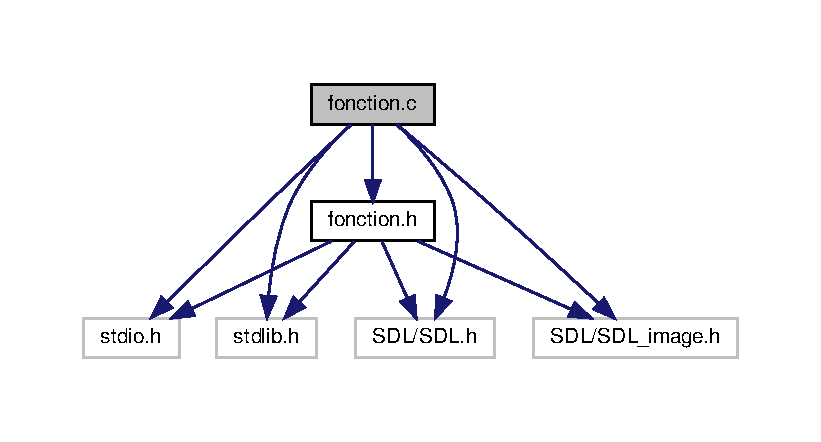
\includegraphics[width=350pt]{fonction_8c__incl}
\end{center}
\end{figure}
\subsection*{Functions}
\begin{DoxyCompactItemize}
\item 
void \hyperlink{fonction_8c_ad8e85dcf2cfe9e95324c056906e25c19}{initialiser\+Obj} (\hyperlink{structObjet}{Objet} $\ast$obj, char name\mbox{[}$\,$\mbox{]}, int x, int y)
\begin{DoxyCompactList}\small\item\em To initialiser object . \end{DoxyCompactList}\item 
\mbox{\Hypertarget{fonction_8c_a33ac93d4cbcb8ad19cce6f86dde40ade}\label{fonction_8c_a33ac93d4cbcb8ad19cce6f86dde40ade}} 
void {\bfseries affichage\+Obj} (\hyperlink{structObjet}{Objet} obj, S\+D\+L\+\_\+\+Surface $\ast$screen)
\item 
int \hyperlink{fonction_8c_a7ebe6513ea3048519d01726d54a128c0}{collisionbb} (S\+D\+L\+\_\+\+Rect posj, S\+D\+L\+\_\+\+Rect posobj)
\begin{DoxyCompactList}\small\item\em To collision bounding box. \end{DoxyCompactList}\end{DoxyCompactItemize}


\subsection{Function Documentation}
\mbox{\Hypertarget{fonction_8c_a7ebe6513ea3048519d01726d54a128c0}\label{fonction_8c_a7ebe6513ea3048519d01726d54a128c0}} 
\index{fonction.\+c@{fonction.\+c}!collisionbb@{collisionbb}}
\index{collisionbb@{collisionbb}!fonction.\+c@{fonction.\+c}}
\subsubsection{\texorpdfstring{collisionbb()}{collisionbb()}}
{\footnotesize\ttfamily int collisionbb (\begin{DoxyParamCaption}\item[{S\+D\+L\+\_\+\+Rect}]{posj,  }\item[{S\+D\+L\+\_\+\+Rect}]{posobj }\end{DoxyParamCaption})}



To collision bounding box. 


\begin{DoxyParams}{Parameters}
{\em posj} & \\
\hline
{\em posobj} & \\
\hline
\end{DoxyParams}
\begin{DoxyReturn}{Returns}
integer 
\end{DoxyReturn}
\mbox{\Hypertarget{fonction_8c_ad8e85dcf2cfe9e95324c056906e25c19}\label{fonction_8c_ad8e85dcf2cfe9e95324c056906e25c19}} 
\index{fonction.\+c@{fonction.\+c}!initialiser\+Obj@{initialiser\+Obj}}
\index{initialiser\+Obj@{initialiser\+Obj}!fonction.\+c@{fonction.\+c}}
\subsubsection{\texorpdfstring{initialiser\+Obj()}{initialiserObj()}}
{\footnotesize\ttfamily void initialiser\+Obj (\begin{DoxyParamCaption}\item[{\hyperlink{structObjet}{Objet} $\ast$}]{obj,  }\item[{char}]{name\mbox{[}$\,$\mbox{]},  }\item[{int}]{x,  }\item[{int}]{y }\end{DoxyParamCaption})}



To initialiser object . 


\begin{DoxyParams}{Parameters}
{\em obj} & \\
\hline
{\em name} & \\
\hline
{\em x} & \\
\hline
{\em y} & \\
\hline
\end{DoxyParams}
\begin{DoxyReturn}{Returns}
Nothing 
\end{DoxyReturn}

\hypertarget{main_8c}{}\section{main.\+c File Reference}
\label{main_8c}\index{main.\+c@{main.\+c}}


Testing Program.  


{\ttfamily \#include $<$stdio.\+h$>$}\newline
{\ttfamily \#include $<$stdlib.\+h$>$}\newline
{\ttfamily \#include $<$S\+D\+L/\+S\+D\+L.\+h$>$}\newline
{\ttfamily \#include $<$S\+D\+L/\+S\+D\+L\+\_\+image.\+h$>$}\newline
{\ttfamily \#include \char`\"{}fonction.\+h\char`\"{}}\newline
Include dependency graph for main.\+c\+:
\nopagebreak
\begin{figure}[H]
\begin{center}
\leavevmode
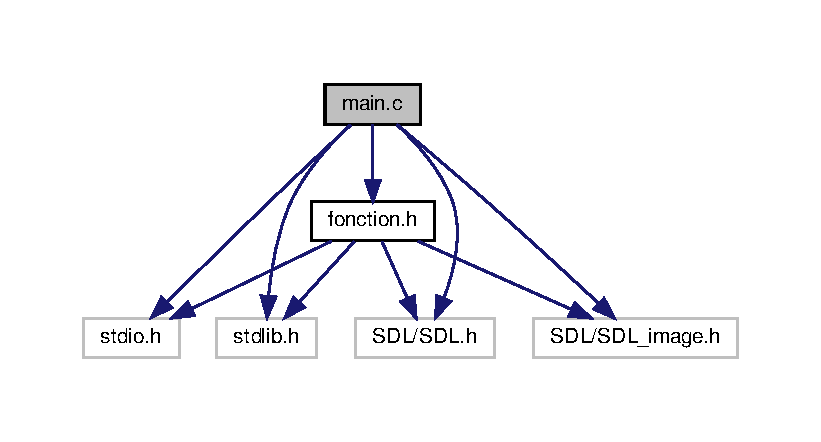
\includegraphics[width=350pt]{main_8c__incl}
\end{center}
\end{figure}
\subsection*{Functions}
\begin{DoxyCompactItemize}
\item 
\mbox{\Hypertarget{main_8c_ae66f6b31b5ad750f1fe042a706a4e3d4}\label{main_8c_ae66f6b31b5ad750f1fe042a706a4e3d4}} 
int {\bfseries main} ()
\end{DoxyCompactItemize}


\subsection{Detailed Description}
Testing Program. 

\begin{DoxyAuthor}{Author}
A\+N\+O\+UN Y\+O\+U\+S\+S\+EF 
\end{DoxyAuthor}
\begin{DoxyVersion}{Version}
0.\+1 
\end{DoxyVersion}
\begin{DoxyDate}{Date}
Apr 01, 2019
\end{DoxyDate}
Testing program for collision bounding box 
%--- End generated contents ---

% Index
\backmatter
\newpage
\phantomsection
\clearemptydoublepage
\addcontentsline{toc}{chapter}{Index}
\printindex

\end{document}
